\documentclass[12pt, a4paper]{article}

\input{~/Desktop/Studia/LaTeX/setup_eng}
\author{Wojciech Orłowski}
\title{The \texttt{KWANT} package – electron transport simulations in magnetic field}
\date{\today}

\begin{document}
\maketitle

\section*{Introduction}

Calculation of properties of quantum transport may be time consuming.
But defining system and method can be made very versatile.
In order to avoid wasting time for code reproduction \texttt{Kwant} has been created.
\texttt{Kwant} is library for \texttt{Python} which allows us to easily create, define and calculate transport properties of quantum system.
This is introductory laboratory to \texttt{Kwant} package.

\section*{Scattering potential}

Prepared part of code was changed to apply potential in the system.
The harmonic potential was centered in the middle of nanowire.
Some transport properties of system have been calculated - conductace (\ref{fig:ex1_conductance}), wavefunctions and current density (\ref{fig:ex1_wavefunctions}).
The system has been presented on figure \ref{fig:ex1_system}.

\begin{figure}[h]
    \begin{center}
        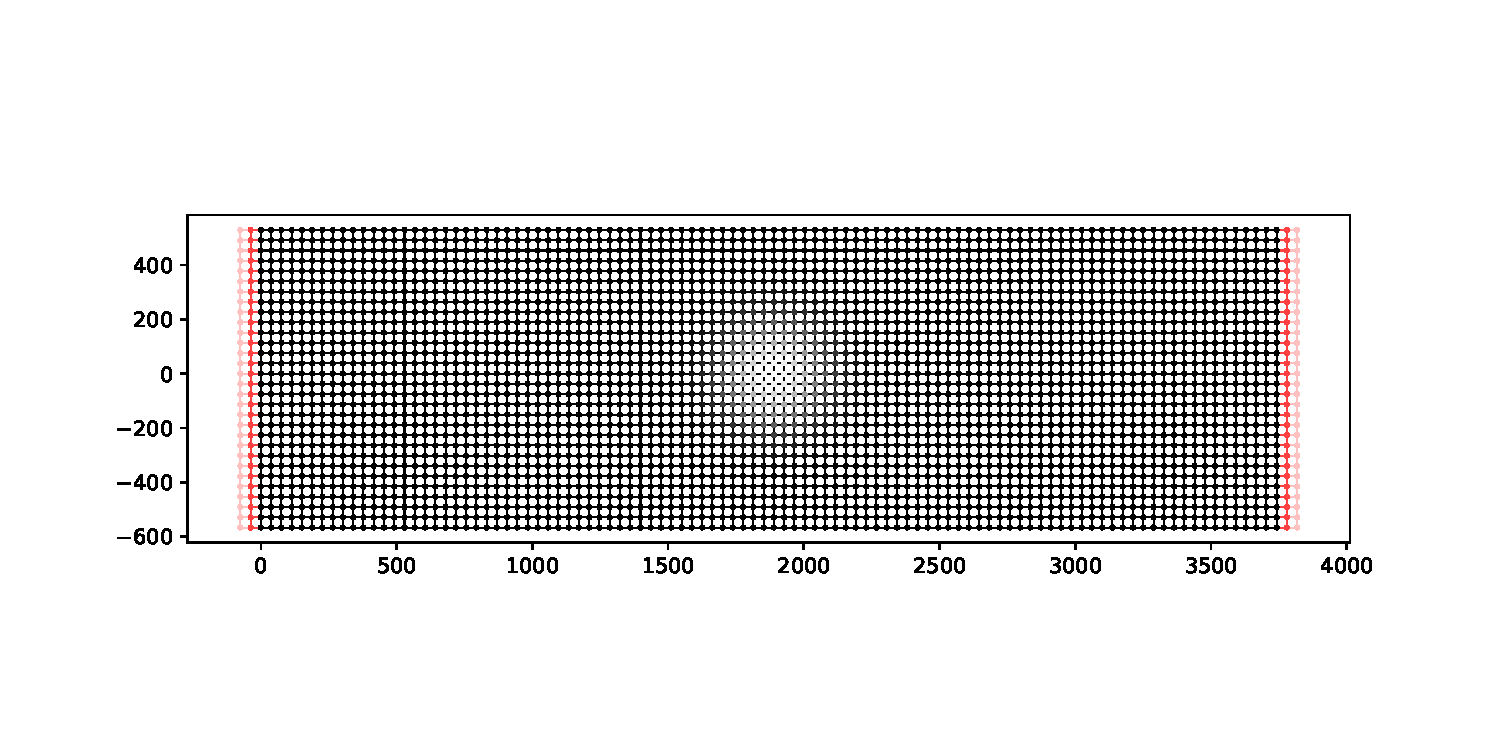
\includegraphics[width=0.95\textwidth]{../plots/kwant_system_with_gauss.pdf}
    \end{center}
    \caption{Quantum wire with colored scattering harmonic potential.}\label{fig:ex1_system}
\end{figure}

\newpage
\begin{figure}[h]
    \begin{center}
        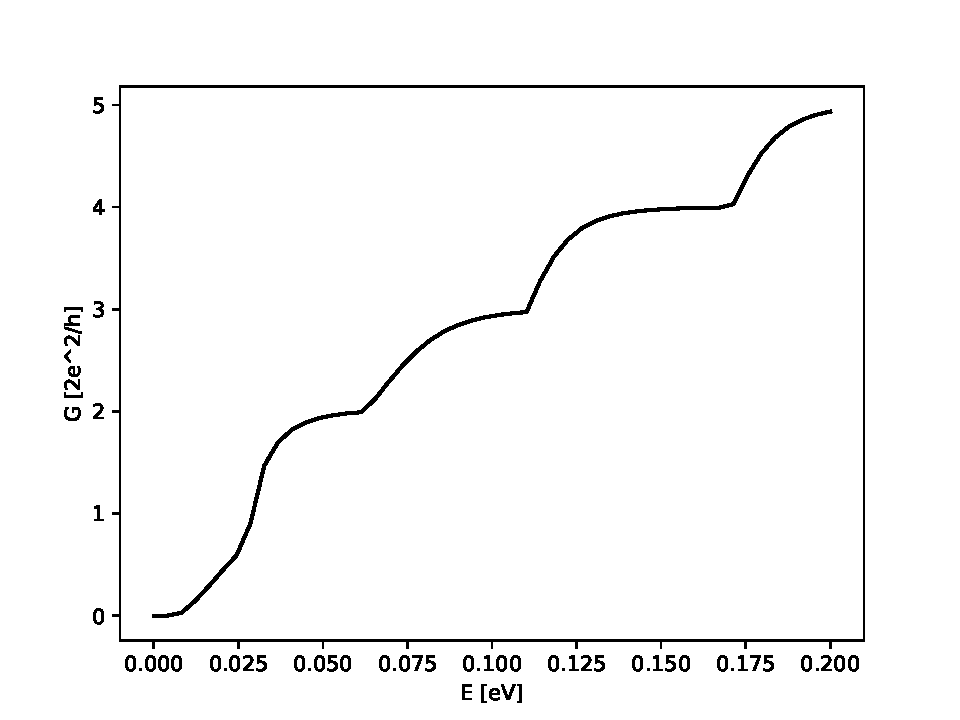
\includegraphics[width=0.95\textwidth]{../plots/condutance.pdf}
    \end{center}
    \caption{Conductance as a function of electron energy.}
    \label{fig:ex1_conductance}
\end{figure}

\begin{figure}[H]
    \begin{center}
        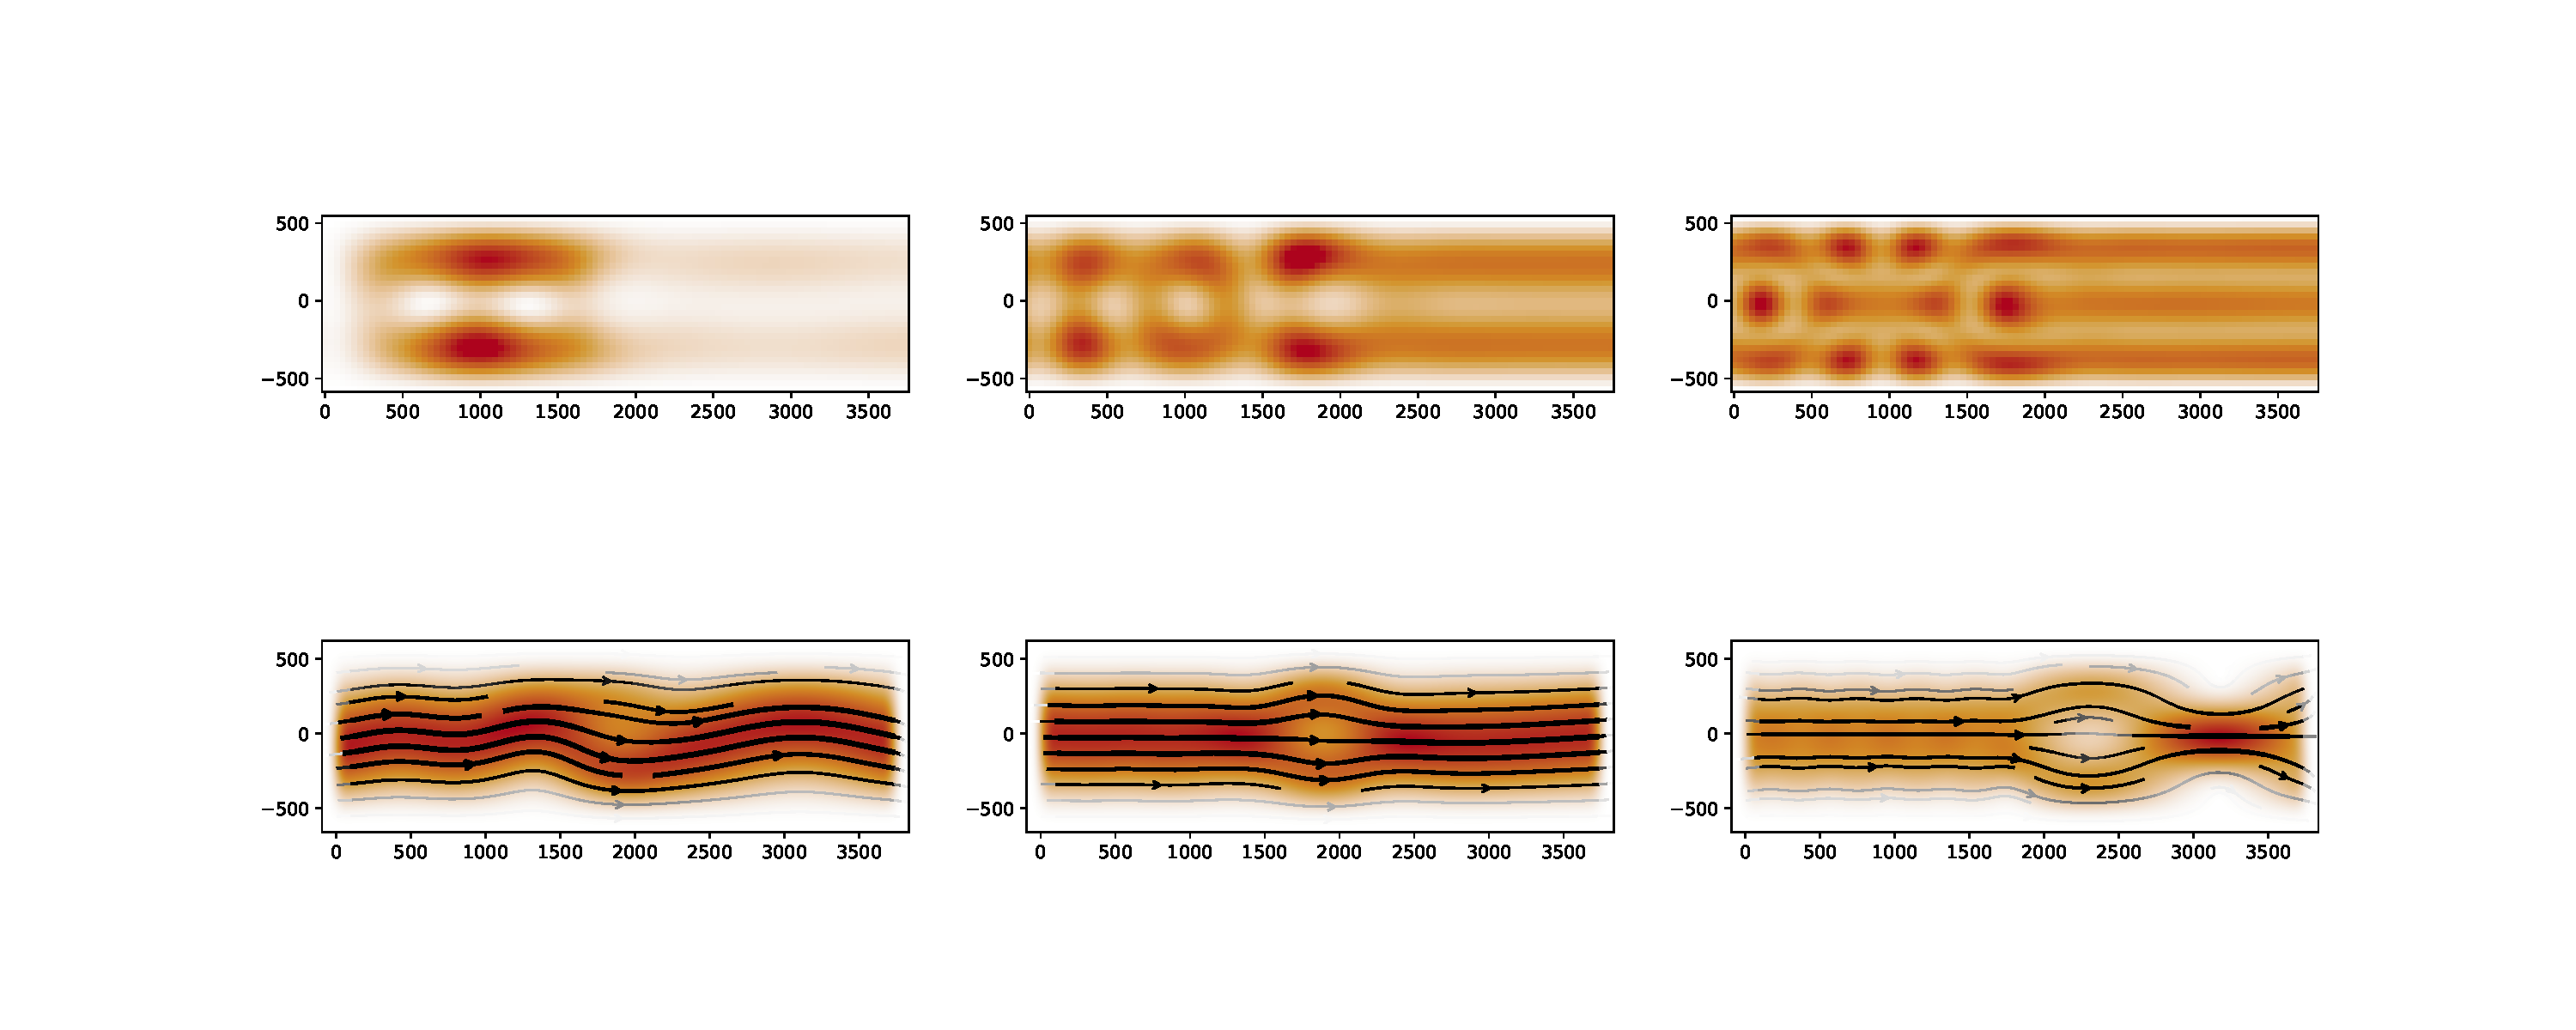
\includegraphics[width=0.95\textwidth]{../plots/wavefunctions_currents.pdf}
    \end{center}
    \caption{Wavefunctions (top) and currents densities(bottom) of electron in nanowire system.}
    \label{fig:ex1_wavefunctions}
\end{figure}

We can see characteristic steps of conductance.
Those steps however are not so steep but rounded.
In the plots of wavefunctions and current densities effect of scattering potential is observable.

\section*{External magnetic field}

In next task scattering potential were removed and effect from transverse magnetic field was added.
Using gauge in form of 
\[ \mathbf{A} = \left( -yB_z, 0, 0 \right) \]
Peierls phase was derived as
\[ P = \exp\left( i \frac{e}{\hbar} \int_{r_n}^{r_m} \mathbf{A}(\vb{r'}) \dd\vb{r'} \right) \rightarrow t_{n,m}\exp\left( -\frac{i}{2}B(x_m - x_n)(y_m + y_n) \right) \]

Obtained dispersion relations for two widths of nanowire were displayed at fig. \ref{fig:ex2_disp}.
Calculated conductance in such system with magnetic field has been shown in fig. \ref{fig:ex2_conductance}.

\begin{figure}[H]
    \begin{center}
        \begin{subfigure}{0.49\textwidth}
            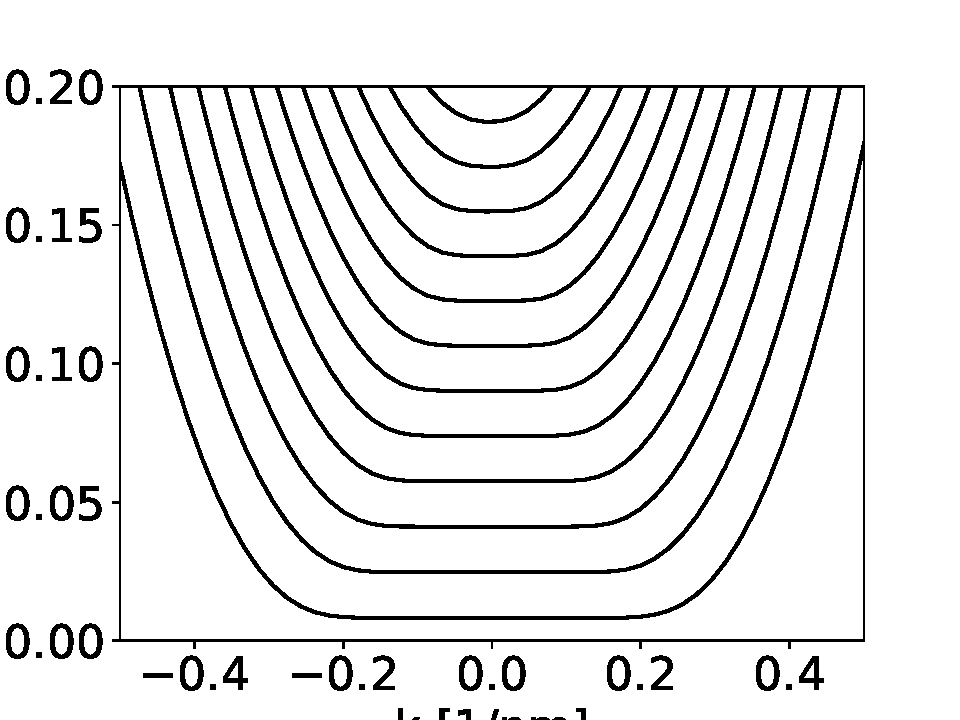
\includegraphics[width=0.95\textwidth]{../plots/disp_ex2_B2_100nm.pdf}
            \caption{}
        \end{subfigure}
        \begin{subfigure}{0.49\textwidth}
            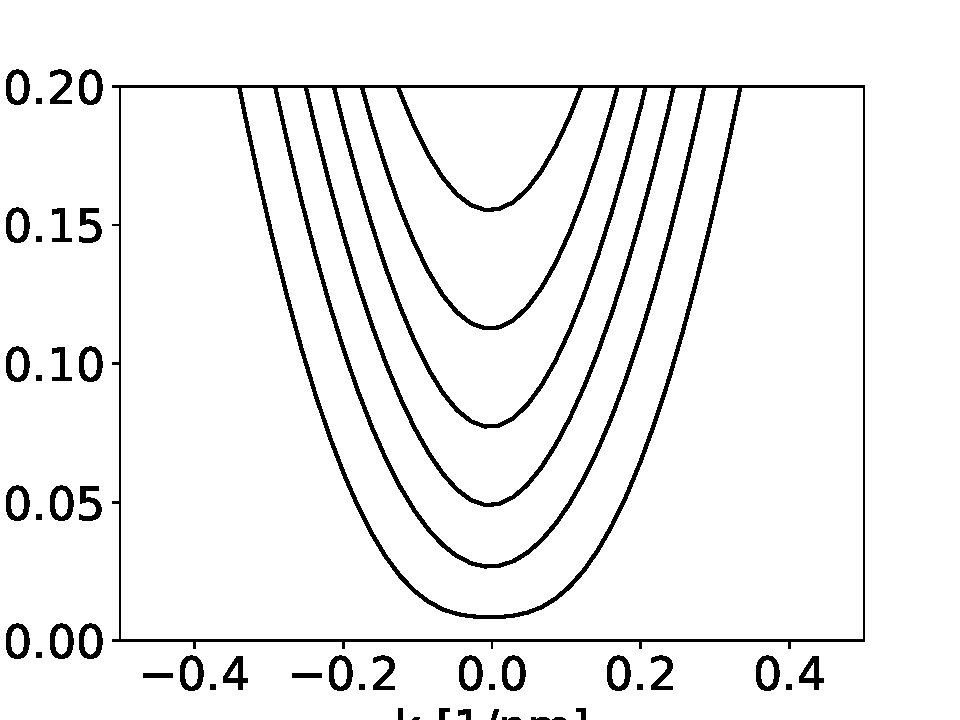
\includegraphics[width=0.95\textwidth]{../plots/disp_ex2_B2_40nm.pdf}
            \caption{}
        \end{subfigure}
    \end{center}
    \caption{Dispersion relation for two widths of nanowire (a) $2W = 200$ nm, (b) $2W = 80$ nm.}
    \label{fig:ex2_disp}
\end{figure}

From this two dispersion relations we can observe that for wider nanowire there for low wavevectors value group velocities are zero.
It is connected with quantum hall effect.
Current is mainly carried in edge states.
For narrower nanowire the effect is lesser.

\begin{figure}[h]
    \begin{center}
        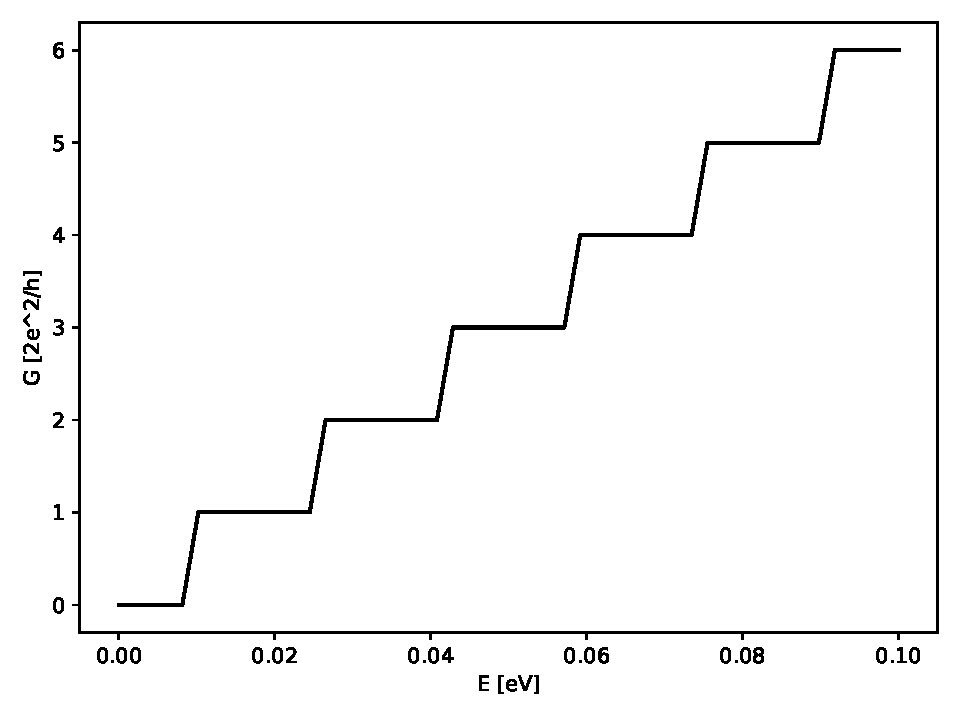
\includegraphics[width=0.95\textwidth]{../plots/ex2_condutance.pdf}
    \end{center}
    \caption{Conductance as a function of electron energy, external magnetic field $B_z = 2$ T, and nanowire width  $2W = 200$ nm.}
    \label{fig:ex2_conductance}
\end{figure}

In conductance plot characteristic steps are visible.
In fig. \ref{fig:ex2_wavefunction} wave function of electron at the lowest state has been presented.

\begin{figure}[H]
    \begin{center}
        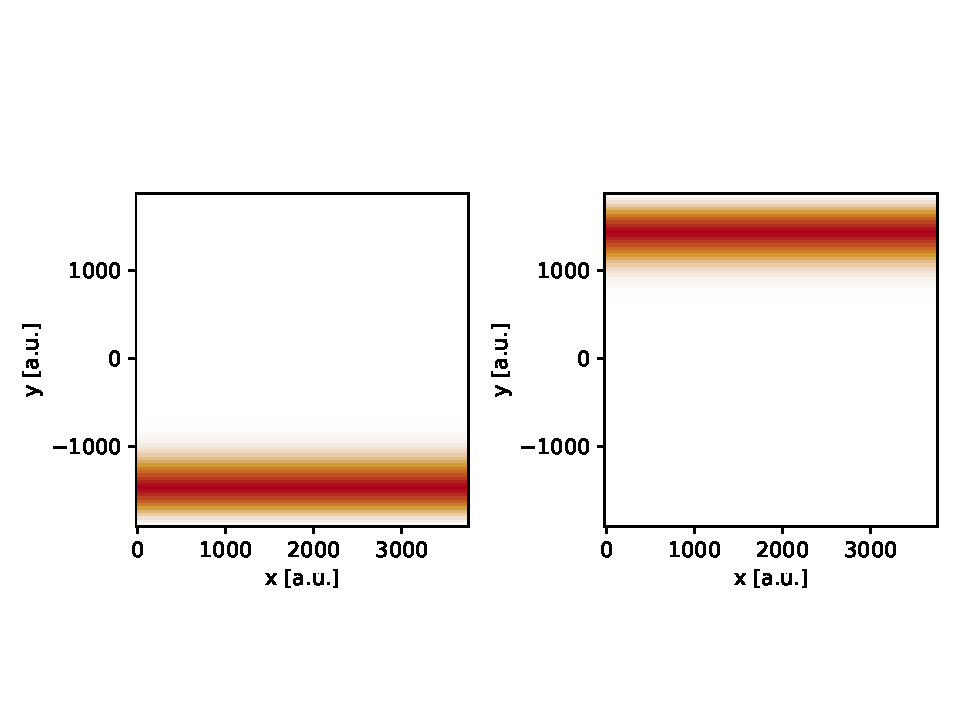
\includegraphics[width=0.95\textwidth]{../plots/ex2_wavefunction.pdf}
    \end{center}
    \caption{Conductance as a function of electron energy, left - electron is input from left, right - electron is input from right. $B_z = 2$ T, $2W = 100$ nm, electron energy is equal to 0.1 eV.}
    \label{fig:ex2_wavefunction}
\end{figure}

\subsection*{Y-shaped junction}

More complicated geometry of system was introduced.
Y-shaped junction is system with one input, which parts into to ways in shape of half a ring.
In the end of each ways there are output leads - bottom and top one.
Whole system has been presented in fig. \ref{fig:ex3_system}

\begin{figure}[H]
    \begin{center}
        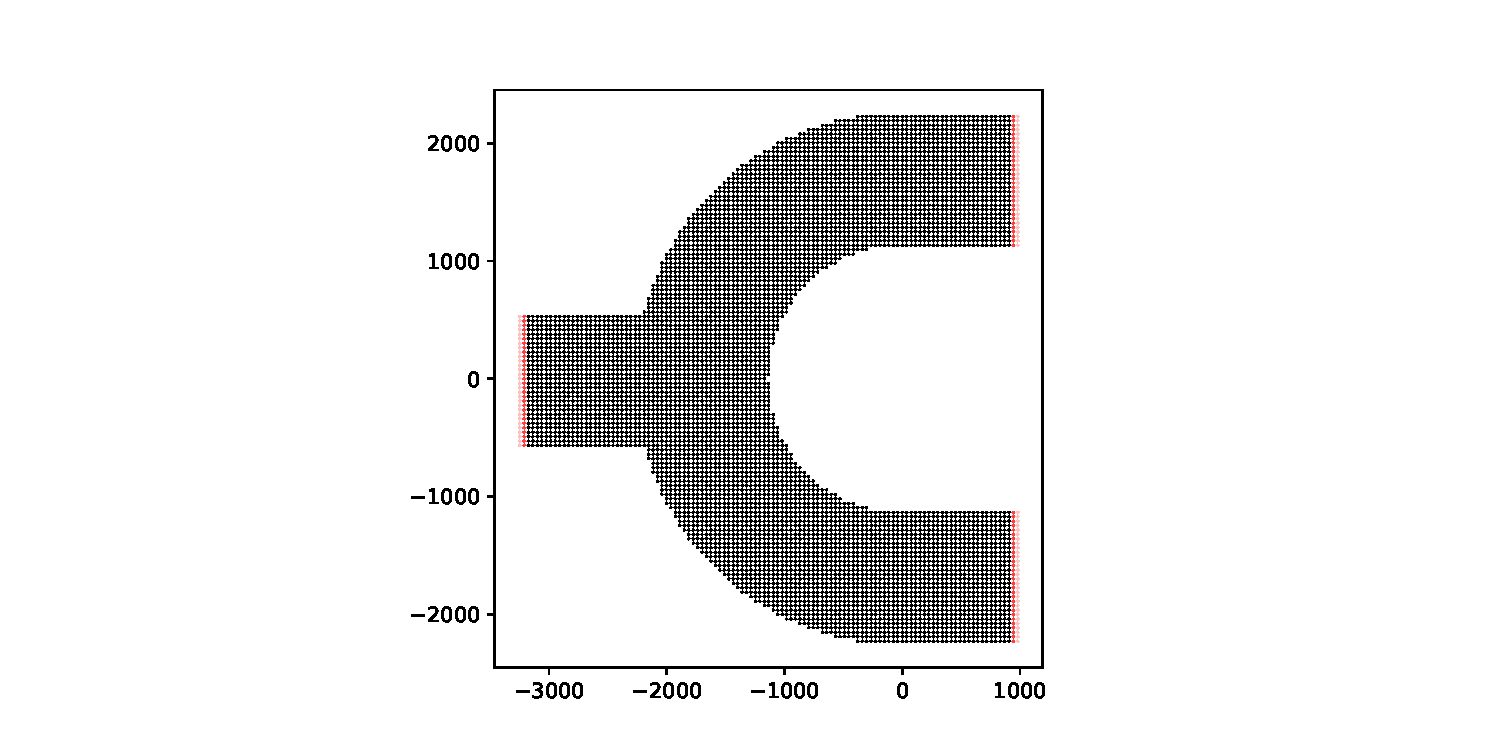
\includegraphics[width=0.8\textwidth]{../plots/kwant_ex3_ring_system.pdf}
    \end{center}
    \caption{Y shaped junction used in calculations. Inner radius of ring is equal to 60 nm, and outer one is equal to 120 nm.}\label{fig:ex3_system}
\end{figure}

Dispersion relation in the left channel at zero magnetic field has been calculated (fig. \ref{fig:ex3_disp})

\begin{figure}[h]
    \begin{center}
        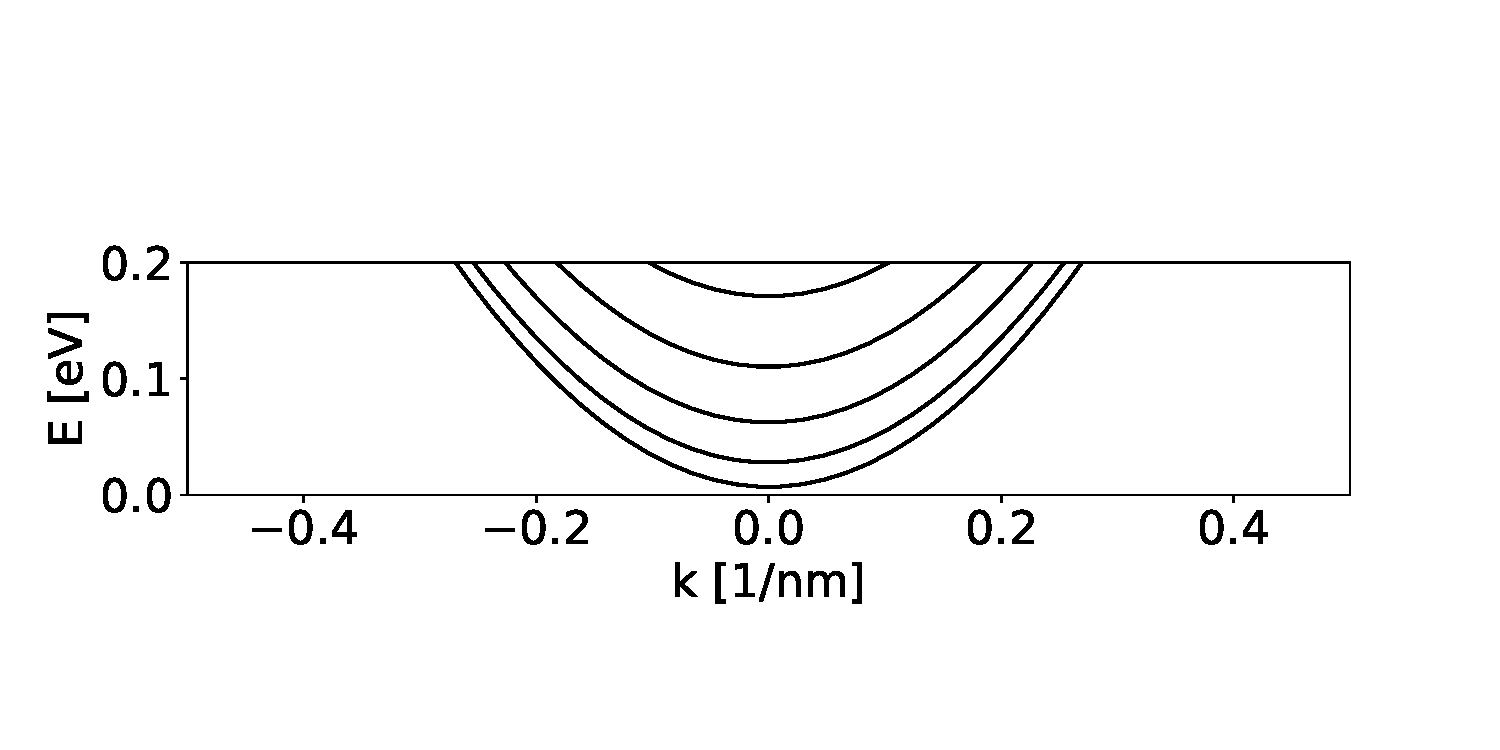
\includegraphics[width=0.95\textwidth]{../plots/kwant_ex3_dispersion.pdf}
    \end{center}
    \caption{Dispersion relation at left channel $B_z$ = 0.}
    \label{fig:ex3_disp}
\end{figure}

Conductance from to both outer leads has been calculated as a function of changing magnetic field (fig. \ref{fig:ex3_cond}).

\begin{figure}[H]
    \begin{center}
        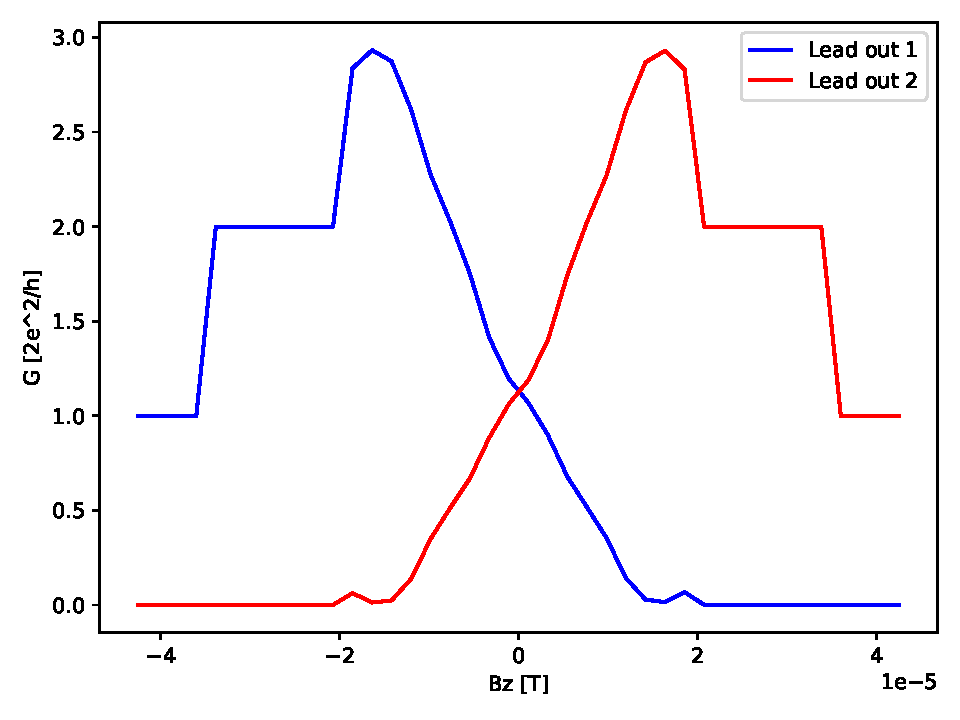
\includegraphics[width=0.95\textwidth]{../plots/conductance_ex3.pdf}
    \end{center}
    \caption{Conductance from the left lead to the upper and lower right lead as a function of magnetic field. Electron energy was set to 0.1 eV.}
    \label{fig:ex3_cond}
\end{figure}

We can observe that by manipulating magnetic field we can force current to go through one of the leads.

Finally current densities at different values of magnetic field were calculated (fig. \ref{fig:ex3_currents}).

\begin{figure}[H]
    \begin{center}
        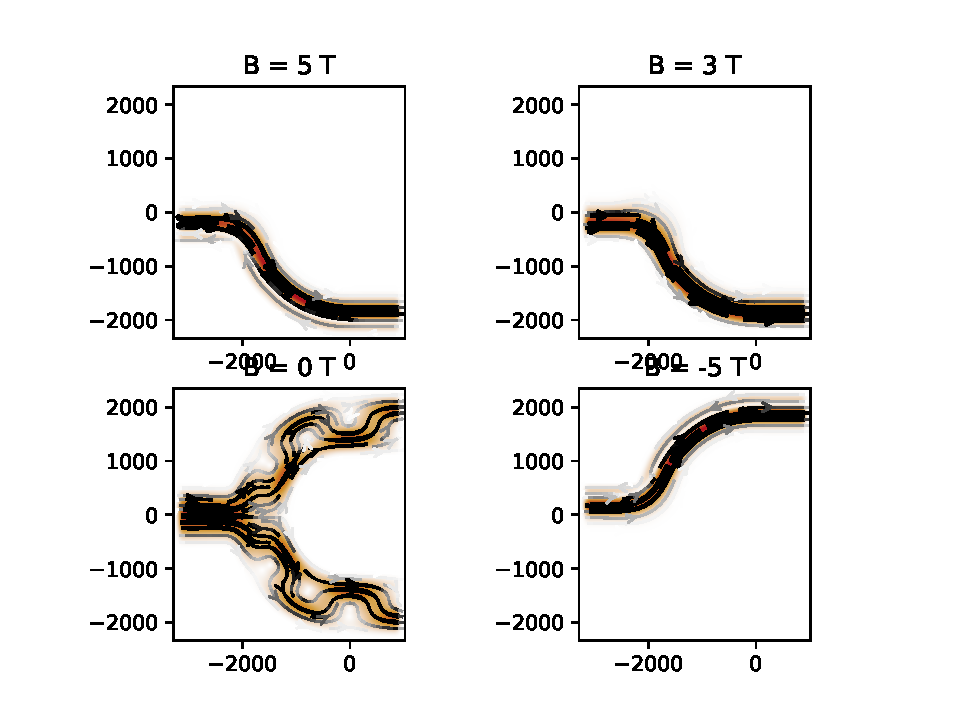
\includegraphics[width=0.95\textwidth]{../plots/current_ex3.pdf}
    \end{center}
    \caption{Current density maps at selected $B_z$ for 1st mode. The incident electron energy was equal to 0.1 eV.}
    \label{fig:ex3_currents}
\end{figure}

At this current density maps we can see the effect of magnetic field and Quantum Hall Effect.
For zero magnetic field current density is equal at the two ways of current.

\section*{Summary}

Using \texttt{KWANT} package allowed us with few lines of python code to calculate very advanced properties of quantum system.
Even for more advanced geometry of system properties were fastly and easily calculated.

\end{document}
